\section{Results}
\begin{figure}[h]
    \centering
    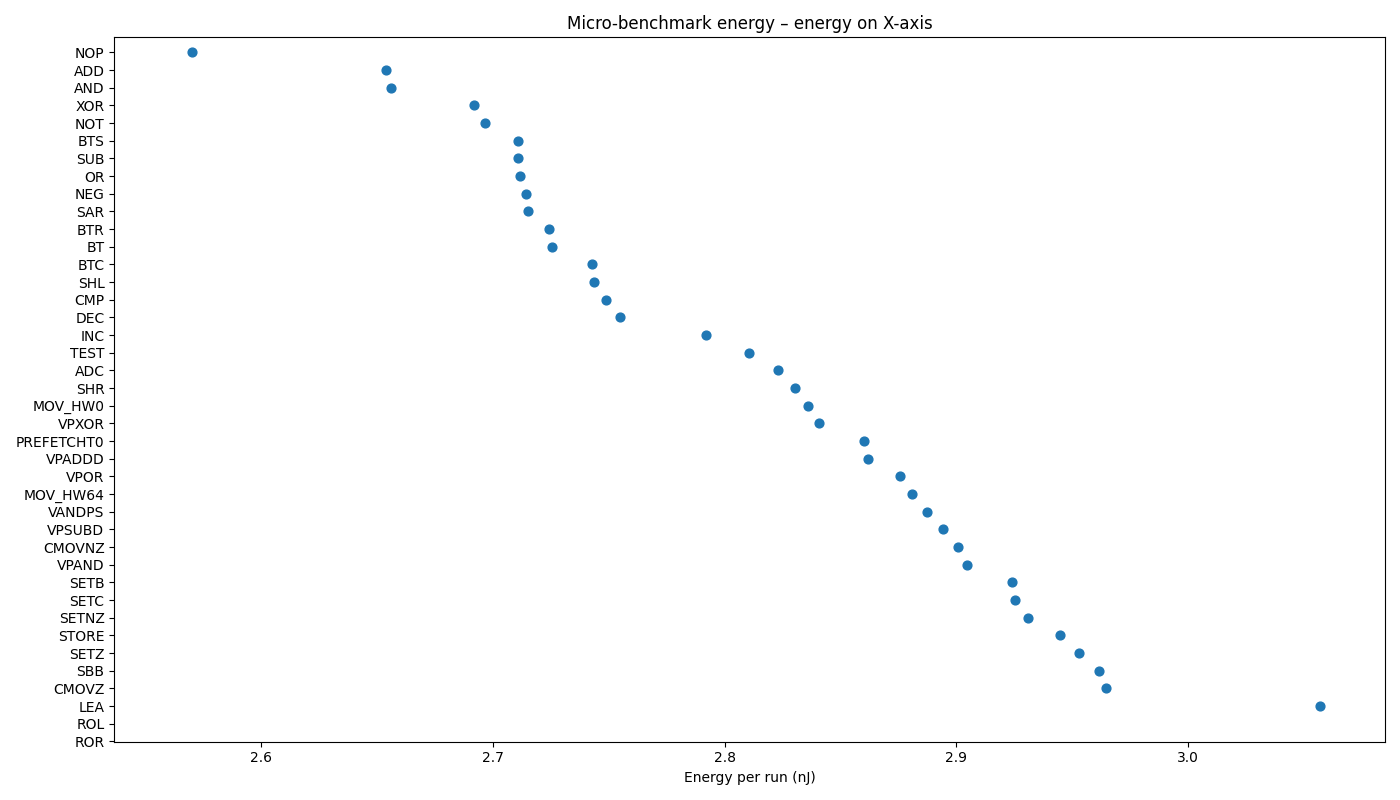
\includegraphics[width=1\linewidth]{Assignment2- Writing a Research Paper in Latex/Images/Instructions_Energy_Readings.png}
    \caption{Energy Consumption Profile of Various x86 Instructions. Each point represents
the energy consumed per run (total/5B) in nJ}
    \label{fig:Instructions_Energy_Readings}
\end{figure}

\begin{table*}[!t]
  \centering
  \begin{tabular}{lccccc}
    \hline
    \textbf{Instruction} & \textbf{Xeon Silver 4214} & \textbf{i7-6700K} & \textbf{i7-8650U} & \textbf{i5-8250U} & \textbf{Xeon Gold 6248} \\
    \hline
    nop                & 0.1795 nJ & 0.1189 nJ & 0.0843 nJ & 0.0912 nJ & 0.1768 nJ \\
    inc r64            & 0.1795 nJ & 0.1208 nJ & 0.0858 nJ & 0.0931 nJ & 0.1781 nJ \\
    xor r64, r64       & 0.1795 nJ & 0.1209 nJ & 0.0849 nJ & 0.0924 nJ & 0.1774 nJ \\
    mov r64, mem       & 0.1868 nJ & 0.1247 nJ & 0.0840 nJ & 0.0950 nJ & 0.1839 nJ \\
    imul r64, r64      & 0.1798 nJ & 0.1169 nJ & 0.0887 nJ & 0.0942 nJ & 0.1792 nJ \\
    fscale             & 0.1867 nJ & 0.1182 nJ & 0.0877 nJ & 0.0963 nJ & 0.1845 nJ \\
    rdrand r64         & 0.1797 nJ & 0.1129 nJ & 0.0982 nJ & 0.1047 nJ & 0.1801 nJ \\
    rdtsc              & 0.1864 nJ & 0.1189 nJ & 0.0848 nJ & 0.0929 nJ & 0.1835 nJ \\
    clflush mem        & 0.1865 nJ & 0.1129 nJ & 0.1018 nJ & 0.1085 nJ & 0.1851 nJ \\
    aesenc xmm, xmm    & 0.1794 nJ & 0.1188 nJ & 0.0946 nJ & 0.1012 nJ & 0.1790 nJ \\
    \hline
  \end{tabular}
  \caption{Per-instruction energy consumption for different Intel processors.
  }
  \label{table:instruction-energy}
\end{table*}

The first and most fundamental experiment was to verify if the foundational leakage pattern of the PLATYPUS attack still exists on a modern, patched processor. The objective was to determine whether the power consumption of different x86 instructions remain distinguishable through the mitigated RAPL interface. If the mitigations were completely effective, we would expect the power consumption to be uniform or for the added noise to overwhelm any signal. We benchmarked 69 instructions for this experiment. We also benchmarked the effect of Hamming Weight on the power consumption of an instruction.

The results strongly suggest that Intel’s RAPL obfuscation, while adding noise,
is insufficient to mask the power variations caused by different CPU operations completely. The data, visualized in Figure \ref{fig:Instructions_Energy_Readings}, reveals a distinct and hierarchical energy profile.
Table \ref{table:instruction-energy} lists the measured energy consumption of different
instructions on our i7-6700K (desktop), Xeon Silver 4214 (server), and i7-8650U (mobile) systems, i5-8250U and Xeon Gold6248. We can clearly
observe inter-instruction differences in energy consumption.